\section{Aplikasi Op-Amp}

\subsection{Pengantar Aplikasi Op-Amp}
\begin{frame}{Pengantar Aplikasi Op-Amp}
	\begin{itemize}
		\item Aplikasi dari op amp sangat luas sekali dan beraneka ragam
		\item Tidak mungkin menjelaskannya secara komprehensif
		\item Sementara kita fokus pada 2 rangkaian dulu.
	\end{itemize}
\end{frame}

\subsection{The Summing Amplifier}
\begin{frame}{The Summing Amplifier}
	\begin{multicols}{2}
		\begin{figure}
			\centering
			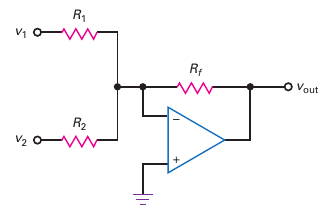
\includegraphics[width=0.9\linewidth]{gambar/fig-16.23a}
			\caption{Rangkaian umming amplifier}
			\label{fig-16.23a}
		\end{figure}
		\begin{itemize}
			\item Menggabungkan 2 atau lebih sinyal analog menjadi satu output
		\end{itemize}
		\columnbreak
		\begin{itemize}
			\item Menguatkan setiap sinyal input
			\item Penguatan setiap channel atau input
			\begin{align*}
				A_{v1(CL)} = \frac{-R_f}{R_1};~~ A_{v2(CL)} = \frac{-R_f}{R_2}
			\end{align*}
			\item Tegangan output
			\begin{equation}\label{pers.16.13}
				v_{out} = A_{v1(CL)}v_1 + A_{v2(CL)} v_2
			\end{equation}
			\item Resistor Thevenin:
			\begin{equation}
				R_{B2} = R_1 \parallel R_2 \parallel R_f \parallel \cdots \parallel R_n
			\end{equation}
		\end{itemize}
	\end{multicols}
\end{frame}

\begin{frame}{The Summing Amplifier}
	\begin{multicols}{2}
		\begin{figure}
			\centering
			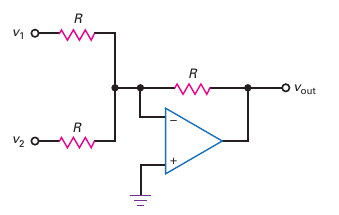
\includegraphics[width=\linewidth]{gambar/fig-16.23b}
			\caption{Rangkaian summing amplifier dengan resistor yang sama}
			\label{fig-16.23b}
		\end{figure}
		\columnbreak
		\begin{itemize}
			\item Tegangan output
			\begin{equation*}
				v_{out} = -(v_1 + v_2 + \cdots + v_n)
			\end{equation*}
		\end{itemize}
	\end{multicols}
\end{frame}

\begin{frame}{The Summing Amplifier}
	\begin{multicols}{2}
		\begin{figure}
			\centering
			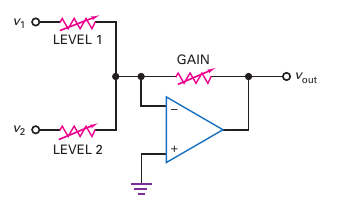
\includegraphics[width=\linewidth]{gambar/fig-16.23c}
			\caption{Rangkaian mixer}
			\label{fig-16.23c}
			\columnbreak
			\begin{itemize}
				\item Menggabungkan sinyal audio
				\item Menurunkan LEVEL 1 $ \rightarrow $ sinyal $ v_1 $ semakin nyaring di output
				\item Menurunkan LEVEL 2 $ \rightarrow $ sinyal $ v_2 $ semakin nyaring di output
				\item Meningkatkan GAIN $ \rightarrow $ kedua sinyal semakin nyaring
			\end{itemize}
		\end{figure}
	\end{multicols}
\end{frame}

\subsection{Voltage Follower}
\begin{frame}{Voltage Follower}
	\begin{multicols}{2}
		\begin{figure}
			\centering
			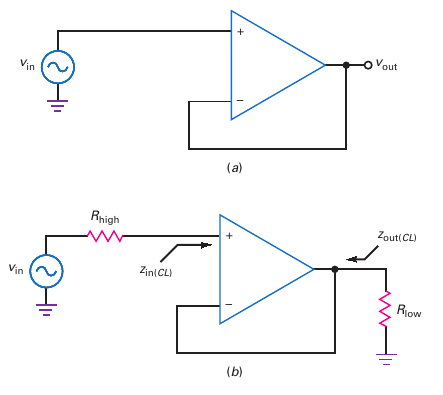
\includegraphics[width=0.9\linewidth]{gambar/fig-16.24}
			\caption{Rangkaian voltage follower}
			\label{fig-16.24}
		\end{figure}
		\columnbreak
		\begin{itemize}
			\item Penguatan tegangan closed-loop:
			\begin{equation}\label{pers.16.15}
				A_{v(CL)} = 1
			\end{equation}
			\item Bandwidth closed-loop:
			\begin{equation}\label{pers.16.16}
				f_{2(CL)} = f_{unity}
			\end{equation}
		\end{itemize}
	\end{multicols}
\end{frame}

\subsection{Contoh Soal 2.12}
\begin{frame}{Contoh Soal 2.12}
	\begin{multicols}{2}
		\begin{center}
			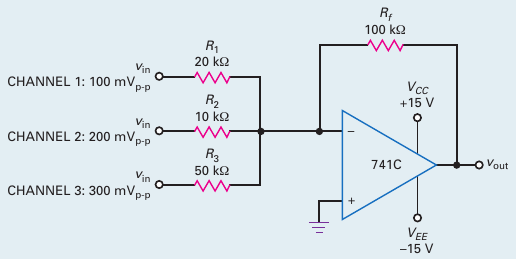
\includegraphics[width=\linewidth]{gambar/fig-16.25}
		\end{center}
		\columnbreak
		\begin{itemize}
			\item Pertanyaan:
			\begin{itemize}
				\item 
			\end{itemize}
		\end{itemize}
	\end{multicols}
\end{frame}